\documentclass[12pt]{article}
\usepackage{amsmath}
\usepackage{mathtools}
\usepackage{bigints}
\usepackage{parskip}
\usepackage{amssymb}

    \newenvironment{myindentpar}[1]%
     {\begin{list}{}%
             {\setlength{\leftmargin}{#1}}%
             \item[]%
     }
     {\end{list}}

\begin{document}
\title{Domain and Range}
\date{}
\author{}
\maketitle

So I noticed a lot of students had trouble on the latest quiz determining the domain of a composition of two functions. So I thought it would be a good idea to write something up discussing domain and range to make things more clear. 

Before we start talking about domain and range let's get an idea of what a function is. A function, $f(x)$ takes numbers as inputs and then it outputs some other number. Visually, that is expressed like this:

\centerline{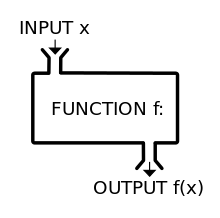
\includegraphics{Function.png}}

So we give the set of inputs a name and we also give the set of outputs a name as well. As you might have guessed they are called the \textbf{domain} and \textbf{range}
\newpage

\textbf{Domain} - the \textit{set of inputs} of a function. In other words, it is all of the values that $x$ can take on

\textbf{Range} - the \textit{set of outputs} of a function. In other words, it is all of the values that $y$ can take on

Now, we will usually just be asked to determine a function's domain. This is often easier than determining the range. But before we start dealing with all of that, let's try to get a sense of what we mean by domain and range with some pretty pictures before we start dealing with boring equations.

You can determine a function's domain by scanning along the x-axis and seeing what values a function does or does not take on. Similarly, we can determine a function's range by scanning along the y-axis to see what values the function does or does not take on. Let's take a look at what I mean with a picture:

\centerline{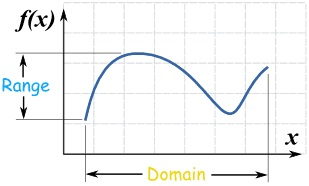
\includegraphics{DomainAndRangePlot.jpg}}

So in the image above we see that the domain of $f(x)$ (the inputs into our function) is contained in some interval along the x-axis and the range of $f(x)$ (the outputs) is contained in some interval along the y-axis. 
\newpage
Let's take a look at some more pictures before we start dealing with equations. Let's take a look at a parabola:
\newline

\centerline{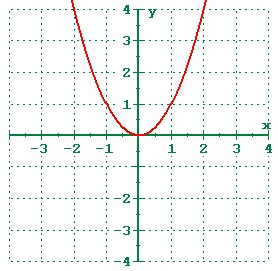
\includegraphics{Quadratic.jpg}}

\textbf{Question:} In the image above, what is the domain and range of this function?

\textbf{Answer:} The \textbf{domain would be all real numbers}. I know it looks like the curve gets cut off at the top of the image, but let's imagine the curve continues going upward forever. Then it does not matter what x-value you give me, it will always be defined.

The \textbf{range} would be $[0, \infty)$ because if we scan along the \textit{y-axis} we see that the values below the line $y = 0$ (this is the x-axis) are never defined.

Let's take a look at a couple more pictures because it's really important to build up some intuition on what exactly we mean by the domain and range before we start dealing with equations.

\centerline{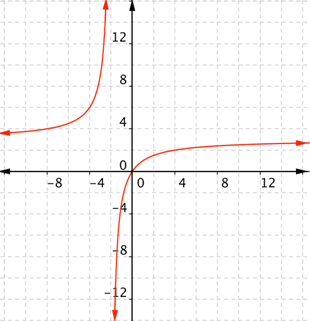
\includegraphics{DomainAndRangePlot2.png}}

\textbf{Question:} What is the domain and range of the function in the image above?

\textbf{Answer:} Again, as we scan along the x-axis we see that the function is not defined for $x=-2$. So the domain in interval notation would be given as $(- \infty, -2) \cup (-2, \infty)$

On the other hand, if we scan along the y-axis we see that the function never takes on the value $y=3$. So the range in interval notation would be given as $(- \infty, 3) \cup (3, \infty)$

And let's take a look at one more picture

\centerline{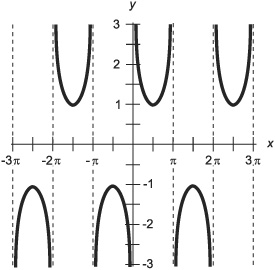
\includegraphics{DomainAndRangePlot3.jpg}}

\textbf{Question:} What is the domain and range of the function in the image above?

\textbf{Answer:} The domain of this function is all x-values except $x = -3 \pi, -2 \pi, - \pi, 0, \pi, 2 \pi, 3 \pi$ 

We could write this in interval notation, but it would be a pain, just know that $x \neq -3 \pi, -2 \pi, - \pi, 0, \pi, 2 \pi, 3 \pi$ gives our domain.

(In fact, this function would continue beyond $x = -3 \pi$ on the left and beyond $x = 3 \pi$ on the right so that $x = n \pi$ is undefined for $n$ being an integer, but that's not very important. I just wanted you to know that this function does not stop just because the image is cut off)

The range of this function is $(- \infty, -1] \cup [1, \infty)$
\newpage

Now let's start getting into some equations. And also, we aren't going to talk about finding the range of a a function unless we deal with that function's graph. Like I said before, finding the range is more difficult than the domain so for simplicity's sake let's just stick to the domain. There are really only two kinds of functions you need to be concerned about at this point in the course:

\begin{enumerate}
\item \textbf{Rational Function}
\item \textbf{Square Root Function}
\end{enumerate}
\hrulefill
\begin{enumerate}
\item \textbf{What is a Rational Function}

By rational function I mean any function that is of the form $\dfrac{P(x)}{Q(x)}$ where both $P(x)$ and $Q(x)$ are a polynomial. 

\textbf{Examples of Rational Functions:}

\begin{enumerate}
\item $y  = x+5$
\item $y = x^2+2x+3$
\item $y = \dfrac{2-x}{x-3}$
\item $y = \dfrac{x^3+2x^2+3x-6}{2-x^2}$
\end{enumerate}

Rational functions are a \textbf{very broad class} of functions, but we only need to be concerned about when that function involves a fraction. And this brings up one of the most important parts about a function involving a fraction. \textbf{You cannot have a zero in the denominator} of a rational function. Most of you I know already knew that, but it's when we start getting into some more complicated examples that this becomes difficult.
\newpage

\textbf{Example 1:} Find the domain of $y = \dfrac{2}{x^2-3x+2}$

\textbf{Answer:} We can't have $0$ in the denominator. So we solve $x^2-3x+2=0$ for x

\hspace{1.1cm}$x^2-3x+2=0$

$\implies (x-2)(x-1) = 0$

$\implies x = 2$ and $x=1$

\textbf{Domain:} $x \neq 1,2$ or, in interval notation, $(-\infty,1) \cup (1,2) \cup (2, \infty)$

\textbf{Try Some Yourself:} Find the domain of the following functions:

\begin{enumerate}
\item $y = x-2$
\item $y = x^2+x-12$
\item $y = \dfrac{1}{x-1}$
\item $y = \dfrac{5}{x^2-8x-20}$
\item $y = \dfrac{x+2}{x^2-9}$
\item $y = \dfrac{x^2-6x+2}{(x^2-16)(x-1)}$
\end{enumerate}
\hrulefill
\item \textbf{What is a Square Root Function?}

A square root function is of the form $y = \sqrt{x}$

The key thing here with the domain is this: \textbf{We cannot have a negative number underneath the $\sqrt{\hspace{1em}}$ symbol}

Any positive number or zero is OK to have underneath the $\sqrt{\hspace{1em}}$, but \textbf{NOT a negative number}. Let's do some examples
\newpage
\textbf{Example 2:} Find the domain of $y = \sqrt{2x-8}$

\textbf{Answer:} 

Remember: \textbf{we cannot have a negative number under the $\sqrt{\hspace{1em}}$ symbol}

So we solve the inequality $2x-8 \geq 0$ since we need $2x-8$ to either be positive or zero for any value of x

\hspace{1cm}$2x-8 \geq 0$

\hspace{.65cm}$\implies 2x \geq 8$

\hspace{.8cm}$\implies x \geq 4$

\textbf{Domain:} $x \geq 4$ or $[4, \infty)$

\textbf{Example 3:} Find the domain of $y = \dfrac{1}{\sqrt{x-3}}$

\textbf{Answer:} This time we have a a square root in the denominator. Because we have a square root, we cannot have a negative number underneath the $\sqrt{\hspace{1em}}$, but since it's also in the denominator we cannot have $\sqrt{x-3} = 0$ which is the same thing as solving $x-3 = 0$

So to find the domain we solve

\hspace{.5cm}$x-3 > 0$ \hspace{1cm} (We are simply excluding the $x$-value where $x-3 = 0$)

$\implies x > 3$

\textbf{Domain:} $x > 3$ or $(3, \infty)$
\newpage

\textbf{Example 4:} Find the domain of $y = \dfrac{x-2}{\sqrt{x^2-9}}$

\textbf{Answer:} This one is tricky. Having the $x^2 - 9$ underneath the $\sqrt{\hspace{1em}}$ symbol can be a pain, but let's show you how to solve it. Again we need $x^2 - 9$ to be strictly positive. (Cannot be zero or negative)

So to find the domain we solve

\hspace{.3cm}$x^2-9 > 0$

$\implies x^2 > 9$

But what does this mean? $x^2>9$ means that the square of the number $x$ must be greater than $9$.

Notice that we have TWO intervals that satisfy this condition: $x<-3$ AND $x>3$

\textbf{Domain:} $x<-3$ or $x > 3$   and in interval notation: $(-\infty, -3) \cup (3, \infty)$

\textbf{Example 5:} Find the domain of $y = \dfrac{\sqrt{x-1}}{x+4}$

\textbf{Answer:} This one can be tricky as well. Notice that we have a square root in the numerator and something else in the denominator.

So to find the domain we solve two things. Let's first deal with the square root.

\hspace{.3cm}$x-1 \geq 0$

$\implies x \geq 1$
 
Now let's deal with the denominator

\hspace{.3cm}$x+4 =0$

$\implies x = -4$

So in summary, these are the conditions on x that we have

Square Root: $x \geq 1$

Denominator: $x \neq -4$

Notice how the condition with the square root satisfies the condition we have from the denominator. If we just have $x \geq 1$, then we are already excluding $x = -4$, so we have our domain. It is...

\textbf{Domain:} $x \geq 1$ or $[1, \infty)$

\textbf{Try Some Yourself:} Find the domain of the following functions:

\begin{enumerate}
\item $y = \sqrt{x+6}$
\item $y = \sqrt{3x-7}$
\item $y = \dfrac{1}{\sqrt{2x-3}}$
\item $y = \dfrac{4-x}{\sqrt{x^2-4}}$
\item $y = \dfrac{x^2-7}{\sqrt{x^2-25}}$
\item $y = \dfrac{\sqrt{x-5}}{x+4}$
\item $y = \dfrac{\sqrt{x+9}}{x-1}$
\item $y = \dfrac{\sqrt{x+5}}{x^2-7x+12}$
\end{enumerate}
\end{enumerate}

\textbf{Finding the Domain of a Composition of Two Functions}

Ok, we are almost done, but we just need to touch on one more thing: function composition. We recently went over this, but it was something you all struggled on in the quiz so I'm going to do a couple examples and and give you some problems to try on your own. These problems can be tricky so you want to be careful whenever you are determining the domain of a composition of two functions. Let's get to it...
\newpage

\textbf{Example 6:} Let $f(x) = \sqrt{x-21}$ and $g(x) = x^2-4$. Find a) $(f \circ g)(x)$ and b) $(g \circ f)(x)$ and state the domain of each

a)  $(f \circ g)(x) = \sqrt{(x^2-4)-21}$

\hspace{2.2cm} $= \sqrt{x^2-25}$

Again, remember we solve $x^2-25 \geq 0$ for the domain

$\implies x^2 \geq 25$

$\implies x\leq -5$ or $x \geq 5$

\textbf{Domain:} $(-\infty, -5] \cup [5, \infty)$

b) $(g \circ f)(x) = (\sqrt{x-21})^2-4$

I'm going to stop right here before we simplify this any further and state the domain of  $(g \circ f)(x)$. Notice how  $(g \circ f)(x)$ takes as input $x$, but not just any old $x$. We have to place a restriction on our inputs. Just because the square will cancel the square root \textbf{does not mean} this function can take any value of $x$ as an input. So we need to solve $x-21 \geq 0$

\textbf{Domain:} $x \geq 21$ or $[21, \infty)$

$(g \circ f)(x) =  (\sqrt{x-21})^2-4$

\hspace{1.7cm} $= x - 21 - 4$

\hspace{1.7cm} $= x-25$

This is simply a line,  but with the added restriction that $x \geq 21$. See how these domain and range problems can be tricky now? I'm going to do one more problem and then I think we've seen enough of this. 

\newpage

\textbf{Example 7:} Let $f(x) = \dfrac{1}{x+7}$ and $g(x) = \dfrac{x}{x-4}$. Find $(f \circ g)(x)$ and and state the domain

a)  $(f \circ g)(x) = \dfrac{1}{\dfrac{x}{x-4}+7}$

Now before we continue on I'm going to note right here that we cannot have $x=4$ because of the $\dfrac{x}{x-4}$ term in the denominator. It's important to make note of this now. For those of you who have seen the movie Inception what we have here is an "infraction" (a fraction inside of a fraction). If you've never seen this movie then you can completely ignore what I just said and go out and see the movie. Now let's continue simplifying...

\hspace{2.2cm} $= \dfrac{1}{\dfrac{x}{x-4}+\dfrac{7(x-4)}{x-4}}$

\hspace{2.2cm} $= \dfrac{1}{\dfrac{x}{x-4}+\dfrac{7x-28}{x-4}}$

\hspace{2.2cm} $= \dfrac{1}{\dfrac{8x-28}{x-4}}$

\hspace{2.2cm} $= \dfrac{x-4}{8x-28}$

\hspace{2.2cm} $= \dfrac{x-4}{4(2x-7)}$


\textbf{Domain:} $x \neq 4$ and $x \neq \dfrac{7}{2}$ or $(-\infty, \dfrac{7}{2}) \cup (\dfrac{7}{2},4) \cup (4, \infty)$

\textbf{Try Some Yourself:}  Find a) $(f \circ g)(x)$ and b) $(g \circ f)(x)$ and state the domain of each

\begin{enumerate}
\item $f(x) = \sqrt{x-4}$ and $g(x) = x^2-12$
\item $f(x) = \sqrt{x-3}$ and $g(x) = x^2-33$
\item $f(x) = \sqrt{x+4}$ and $g(x) = \dfrac{1}{x-2}$ (find just $(g \circ f)(x)$)
\item $f(x) = \dfrac{1}{x+6}$ and $g(x) = \dfrac{x}{x-1}$ (find just $(f \circ g)(x)$)
\end{enumerate}











\end{document}